\stepcounter{section}
\section*{\Large\centering {CHAPTER 3 \\ SYSTEM ANALYSIS }}
\addcontentsline{toc}{section}{CHAPTER 3: System Analysis}\label{3}

\subsection{System Analysis}
System analysis is about understanding the problem clearly before building the system. It focuses on finding what the system should do (functional requirements like uploading MRI scans, generating reports) and how well it should perform (non-functional requirements like accuracy, speed, and security). It also checks if the system is technically, operationally, and economically feasible. Finally, analysis uses modeling techniques (like use case and activity diagrams) to show how users and components will interact.
\subsubsection{Requirement Analysis}
\begin{enumerate}[label=\roman*.]
    \item \textbf{Functional Requirements}
          \begin{center}
              \begin{figure}[H]
                  \centering
                  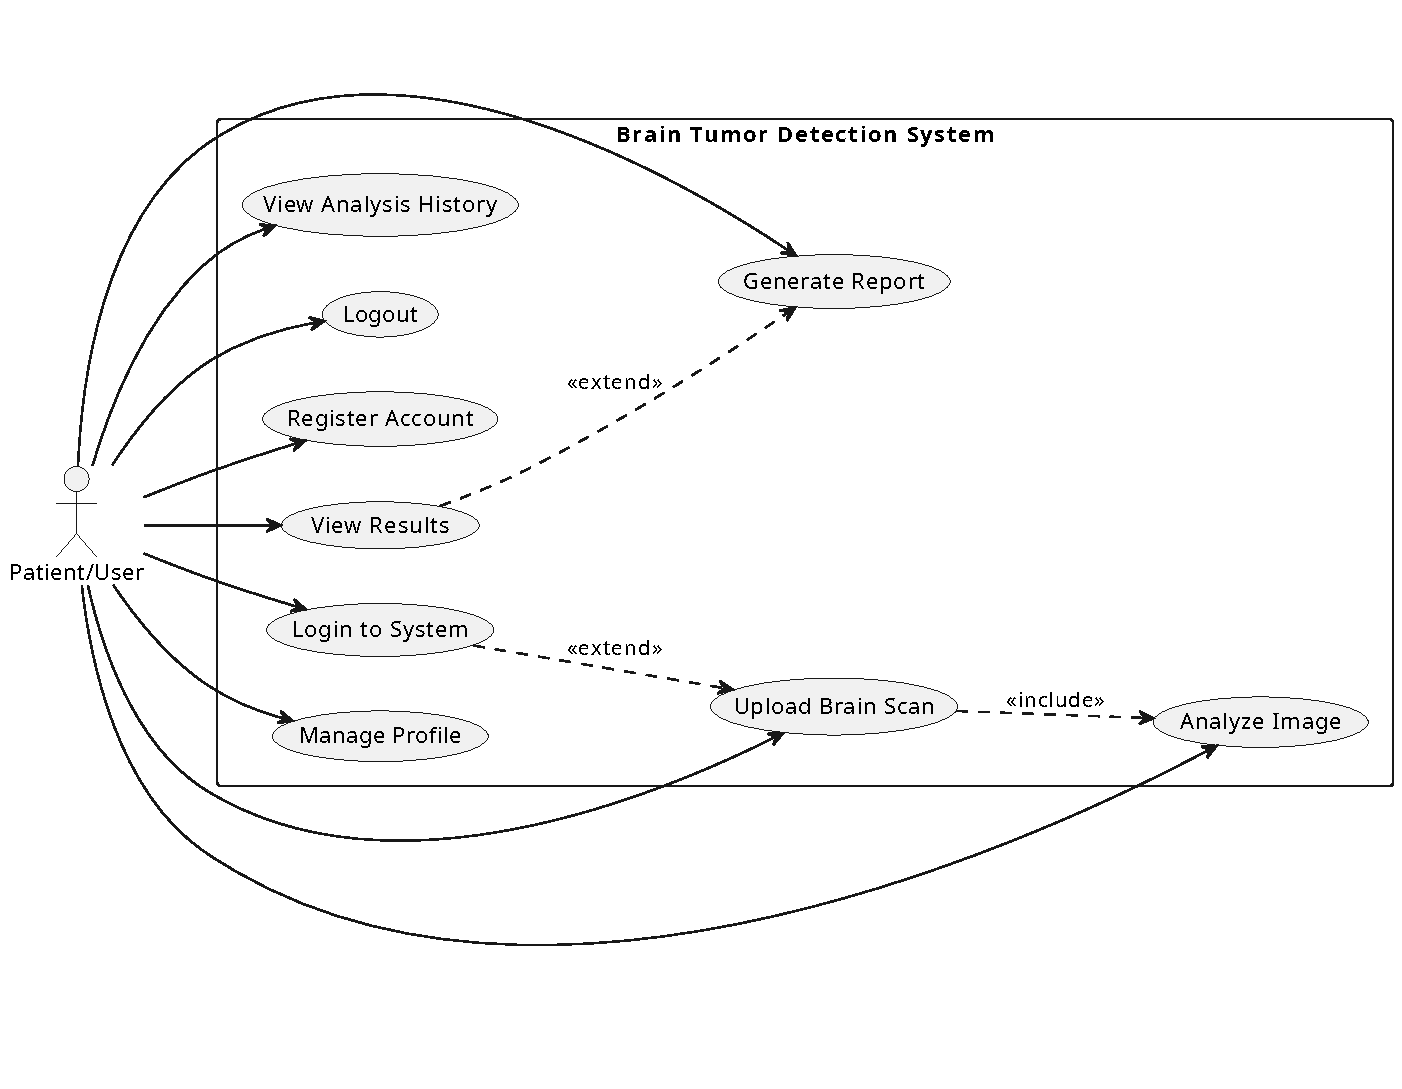
\includegraphics[width=0.85\linewidth]{Images/usecase.pdf}
                  \caption{Use Case Diagram}
                  \label{fig:UseCaseDiagram}
              \end{figure}
          \end{center}
          The use case diagram presents the fundamental interactions between system actors and core functionalities of the application. The primary actor, Patient/User, represents individuals seeking brain tumor analysis services and can perform essential activities including account registration, system login, brain scan upload, image analysis, result viewing, report generation, profile management, analysis history review, and system logout. The diagram establishes key relationships through include and extend dependencies, where uploading brain scans necessarily includes the analysis process, viewing results can optionally extend to report generation, and successful login enables access to upload functionality.

    \item \textbf{Non-Functional Requirements}
          \begin{itemize}
              \item \textbf{Performance:} The system should process MRI images and provide classification results within 10--15 seconds per image, ensuring minimal waiting time for medical practitioners during diagnosis.

              \item \textbf{Accuracy:} The brain tumor classification model must maintain a minimum accuracy of 95\% on test datasets, with precision and recall rates above 90\% for each tumor type (glioma, meningioma, pituitary).

              \item \textbf{Usability:} The user interface must be intuitive and easy to navigate for medical practitioners with varying levels of technical expertise, requiring minimal training for effective system usage.

              \item \textbf{Reliability:} The system should maintain 99.5\% uptime with robust error handling and recovery mechanisms to ensure continuous availability for critical medical applications.

              \item \textbf{Security:} Patient data and medical images must be encrypted during transmission and storage, with secure user authentication to comply with healthcare data protection regulations.

              \item \textbf{Compatibility:} The web-based interface must be compatible with major browsers (Chrome, Firefox, Safari, Edge) and responsive across desktop, tablet, and mobile devices.

              \item \textbf{Maintainability:} The codebase should follow clean coding practices and modular design principles to facilitate future updates, model improvements, and feature additions.

              \item \textbf{Data Integrity:} The system must ensure data consistency and prevent corruption during image upload, processing, and storage operations with appropriate backup and recovery mechanisms.

              \item \textbf{Extensibility:} The system architecture should support future enhancements such as additional imaging modalities (CT scans, X-rays), new tumor types, and integration with existing hospital information systems.
          \end{itemize}

\end{enumerate}
\subsubsection{Feasibility Analysis}
\begin{enumerate}[label=\roman*.]
    \item \textbf{Technical} \\
          The system demonstrates strong technical viability through proven technology integration. The architecture combines React/TypeScript frontend with Node.js/Express backend, providing robust scalability for medical applications. TensorFlow/Keras implementation ensures reliable deep learning capabilities with 90\% accuracy in brain tumor classification. Docker containerization enables consistent deployment across environments, while MongoDB offers flexible medical data storage. JWT authentication and bcrypt encryption meet healthcare security standards. The system supports cross-platform compatibility and future DICOM integration, confirming technical robustness and extensibility for medical imaging workflows.

    \item \textbf{Operational} \\
          The system aligns effectively with existing healthcare workflows and user requirements. The intuitive web-based interface requires minimal training for medical professionals, supporting multiple user roles including patients, doctors, and administrators. Automated analysis reduces interpretation time while maintaining human oversight through confidence scoring. The system integrates seamlessly with existing radiology workflows and generates comprehensive PDF reports for documentation. Cloud deployment supports telemedicine scenarios, while flexible architecture accommodates both individual practitioners and institutional deployments across various healthcare settings.
    \item \textbf{Economic} \\
          The project demonstrates favorable cost-benefit ratios through open-source technology utilization, eliminating expensive licensing fees. Development costs remain manageable with estimated ROI within 18--24 months based on subscription models and pay-per-analysis pricing. The system addresses significant market demand for affordable medical imaging tools, particularly in resource-limited settings. Operational costs scale proportionally with adoption, while revenue potential exists through institutional subscriptions and premium features. Long-term sustainability benefits from cloud scaling and automated operations reducing maintenance overhead.

    \item \textbf{Schedule}
          The four-month development timeline from Jestha through Bhadra provides realistic project completion within allocated resources. Modular architecture enables parallel development streams, while agile methodology ensures continuous progress monitoring. The schedule accommodates comprehensive testing phases and risk mitigation strategies with adequate buffer time for unforeseen challenges. Critical milestones include system design completion, core functionality implementation, thorough testing, and final deployment preparation, ensuring successful delivery within the specified timeframe.
        %   \begin{figure}[H]
        %       \centering
        %       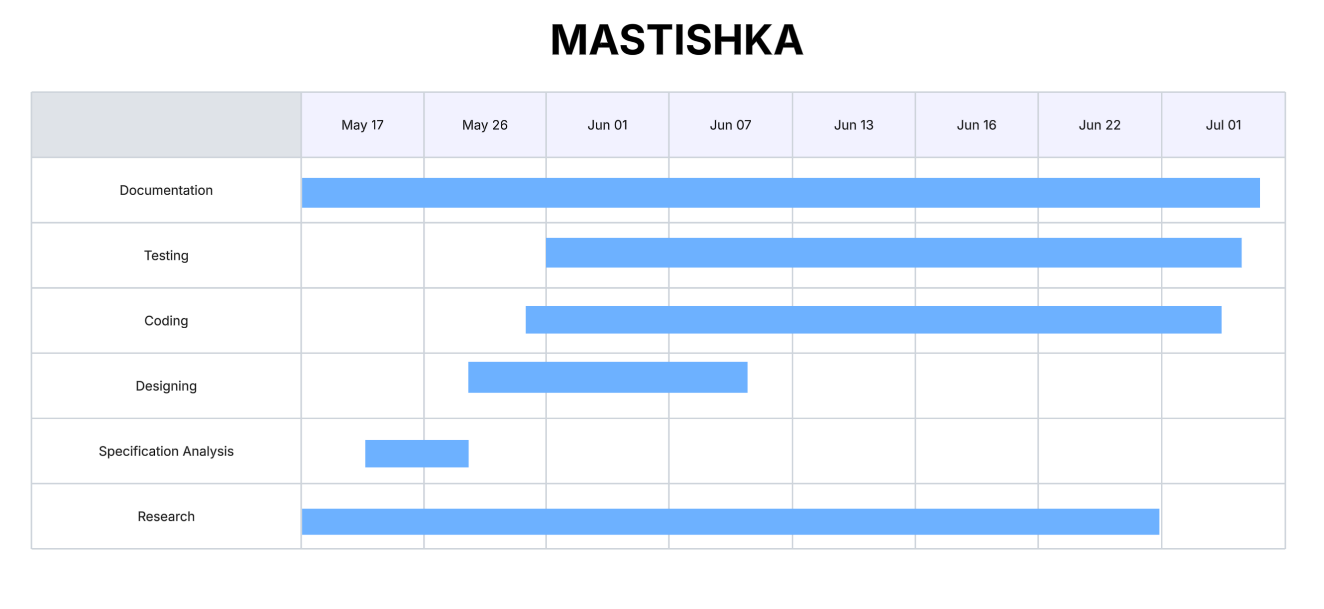
\includegraphics[width=1\linewidth]{Images/gantt.png}
        %       \caption{Sample Gantt Chart demonstrating schedule feasibility}
        %       \label{fig:gantt}
        %   \end{figure}

        \begin{table}[h!]
\centering
\footnotesize
\setlength{\tabcolsep}{2pt}
\resizebox{\textwidth}{!}{%
\begin{tabular}{@{}l*{16}{c}@{}}
\toprule
\multirow{2}{*}{\textbf{Task}} &
\multicolumn{4}{c}{\textbf{Jestha}} &
\multicolumn{4}{c}{\textbf{Ashar}} &
\multicolumn{4}{c}{\textbf{Shawarn}} &
\multicolumn{4}{c}{\textbf{Bhadra}} \\
\cmidrule(lr){2-5}\cmidrule(lr){6-9}\cmidrule(lr){10-13}\cmidrule(lr){14-17}
 & W1 & W2 & W3 & W4 & W1 & W2 & W3 & W4 & W1 & W2 & W3 & W4 & W1 & W2 & W3 & W4 \\
\midrule
Requirement Analysis              & \GantP  & \GantP  &     &     &     &     &     &     &     &     &     &     &     &     &     &     \\
Planning                          &     & \GantP  & \GantP  &     &     &     &     &     &     &     &     &     &     &     &     &     \\
Design                            &     &     & \GantP  & \GantP  & \GantP  & \GantP  &     &     &     &     &     &     &     &     &     &     \\
\addlinespace[2pt]
Iteration 1 — Dev                 &     &     &     &     & \GantD  & \GantD  & \GantD  &     &     &     &     &     &     &     &     &     \\
Iteration 1 — Test                &     &     &     &     &     &     &     & \GantT  &     &     &     &     &     &     &     &     \\
\addlinespace[2pt]
Iteration 2 — Dev                 &     &     &     &     &     &     &     &     & \GantD  & \GantD  & \GantD  &     &     &     &     &     \\
Iteration 2 — Test                &     &     &     &     &     &     &     &     &     &     & \GantT  &     &     &     &     &     \\
\addlinespace[2pt]
Iteration 3 — Dev                 &     &     &     &     &     &     &     &     &     &     & \GantD  & \GantD  & \GantD  &     &     &     \\
Iteration 3 — Test                &     &     &     &     &     &     &     &     &     &     &     &     & \GantT  &     &     &     \\
\addlinespace[2pt]
Iteration 4 — Dev                 &     &     &     &     &     &     &     &     &     &     &     &     & \GantD  & \GantD  & \GantD  &     \\
Iteration 4 — Test                &     &     &     &     &     &     &     &     &     &     &     &     &     &     & \GantT  &     \\
\addlinespace[2pt]
Deployment                        &     &     &     &     &     &     &     &     &     &     &     &     &     &     & \GantY  & \GantY  \\
Documentation (ongoing)           & \GantC  & \GantC  & \GantC  & \GantC  & \GantC  & \GantC  & \GantC  & \GantC  & \GantC  & \GantC  & \GantC  & \GantC  & \GantC  & \GantC  & \GantC  & \GantC  \\
\bottomrule
\end{tabular}%
}
\caption{Gantt-style weekly schedule following iterative development. Shaded cells indicate active work.}
\end{table}
\end{enumerate}

\subsubsection{Analysis}
The system is analyzed using the Object-Oriented Approach, which includes three
aspects. Object Modelling with Class and Object Diagrams shows the static
structure of the system. Dynamic Modelling with State and Sequence Diagrams
explains object interactions and state changes. Process Modelling with Activity
Diagrams illustrates the workflow and control flow of operations.
\begin{enumerate}[label=\roman*.]
    \item \textbf{Class Diagram}
          \begin{center}
              \begin{figure}[H]
                  \centering
                  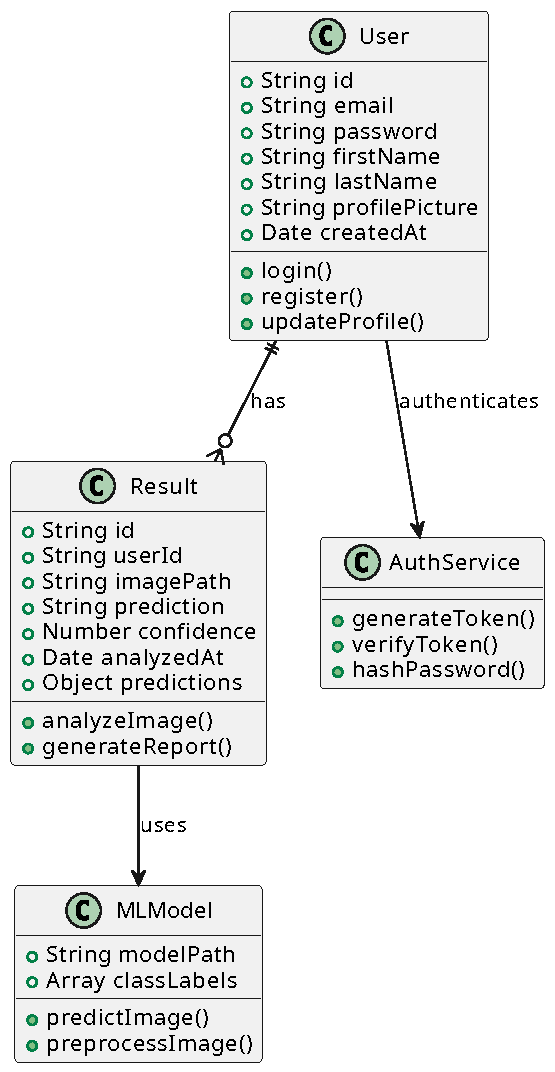
\includegraphics[width=0.4\linewidth]{Images/Highlevel/class.pdf}
                  \caption{Class Diagram}
                  \label{fig:ClassDiagram}
              \end{figure}
          \end{center}
          The class diagram presents the fundamental building blocks of the brain tumor detection system. The User class serves as the central entity representing application users, containing basic authentication and profile information along with methods for login, registration, and profile updates. The Result class captures the outcomes of brain tumor analyses, storing prediction results, confidence scores, and timestamps while providing methods for image analysis and report generation. The MLModel class abstracts the machine learning functionality, encapsulating the model path and class labels with methods for image prediction and preprocessing. The AuthService class handles security operations including token generation, verification, and password hashing. The relationships show that users can have multiple analysis results, results utilize the ML model for predictions, and users interact with the authentication service for security purposes.



    \item \textbf{Object Diagram}
          \begin{center}
              \begin{figure}[H]
                  \centering
                  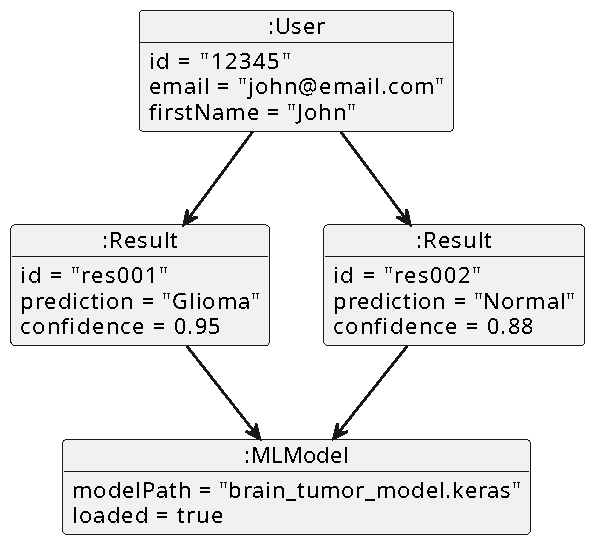
\includegraphics[width=0.60\linewidth]{Images/Highlevel/object.pdf}
                  \caption{Object Diagram}
                  \label{fig:ObjectDiagram}
              \end{figure}
          \end{center}
          This object diagram illustrates a specific runtime scenario where a user named John has performed brain tumor analyses. The diagram shows concrete instances of the classes, with User object ``12345'' representing John's account information, connected to two Result objects showing actual analysis outcomes -- one detecting a Glioma tumor with 95\% confidence and another showing a Normal scan with 88\% confidence. Both results are linked to the same MLModel instance that has successfully loaded the Keras model file. This snapshot demonstrates how the system maintains relationships between users and their analysis history while sharing the ML model instance across multiple predictions.

          \newpage
    \item \textbf{State Diagram}
          \begin{center}
              \begin{figure}[H]
                  \centering
                  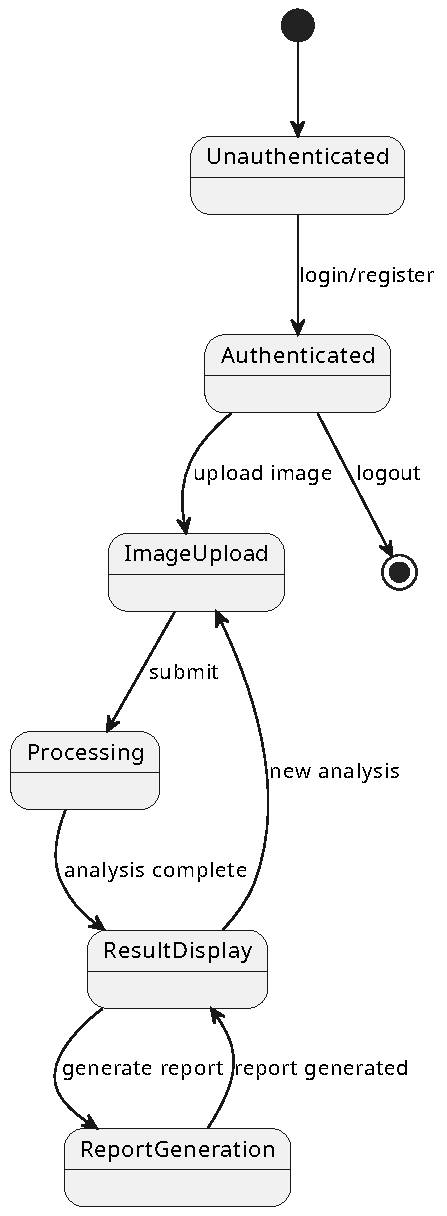
\includegraphics[width=0.35\linewidth]{Images/Highlevel/state.pdf}
                  \caption{State Diagram}
                  \label{fig:StateDiagram}
              \end{figure}
          \end{center}
          The state diagram traces the user journey through the application's main workflow states. Users begin in an unauthenticated state and transition to authenticated status through successful login or registration. Once authenticated, users can navigate to image upload functionality, where they submit brain scan images for analysis. The system then moves to a processing state where the ML model analyzes the uploaded image. Upon completion, users reach the result display state where they can view their analysis outcomes. From this state, users can either initiate new analyses by returning to image upload or generate detailed PDF reports. The diagram also shows the logout transition that returns users to the unauthenticated state, completing the application lifecycle. This workflow represents the essential data flow from image submission to result presentation.


    \item \textbf{Sequence Diagram}
          \begin{center}
              \begin{figure}[H]
                  \centering
                  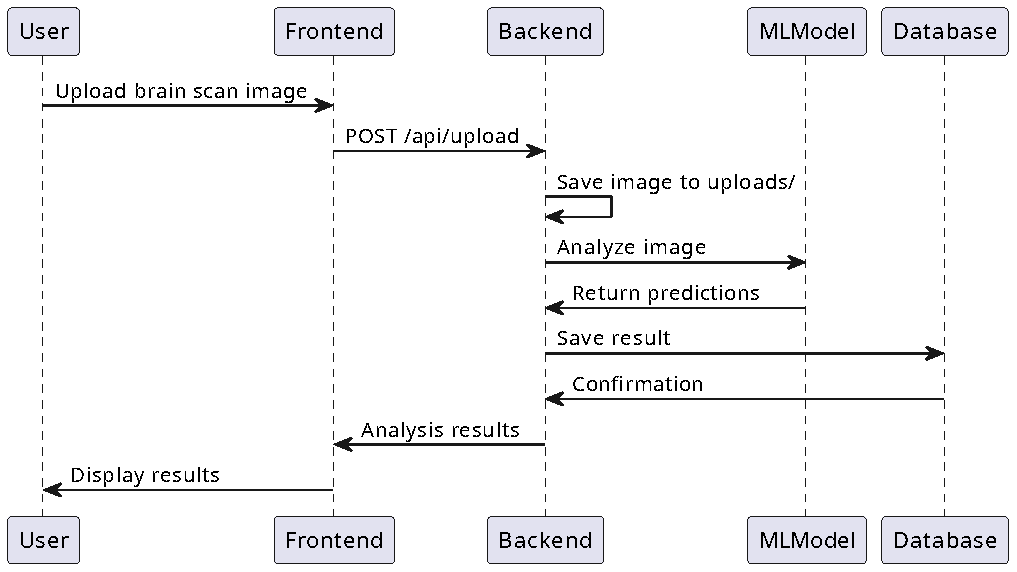
\includegraphics[width=0.9\linewidth]{Images/Highlevel/sequence.pdf}
                  \caption{Sequence Diagram}
                  \label{fig:SequenceDiagram}
              \end{figure}
          \end{center}
          This sequence diagram depicts the core interaction flow for brain tumor analysis. The process begins when a user uploads a brain scan image through the frontend interface. The frontend forwards this request to the backend server, which first saves the uploaded image to the designated uploads directory. The backend then invokes the ML model service to analyze the saved image, receiving prediction results including tumor classification and confidence scores. These results are subsequently stored in the database for future reference and user history. The backend returns the analysis results to the frontend, which presents them to the user in a comprehensible format. This workflow represents the essential data flow from image submission to result presentation.


    \item \textbf{Activity Diagram}
          \begin{center}
              \begin{figure}[H]
                  \centering
                  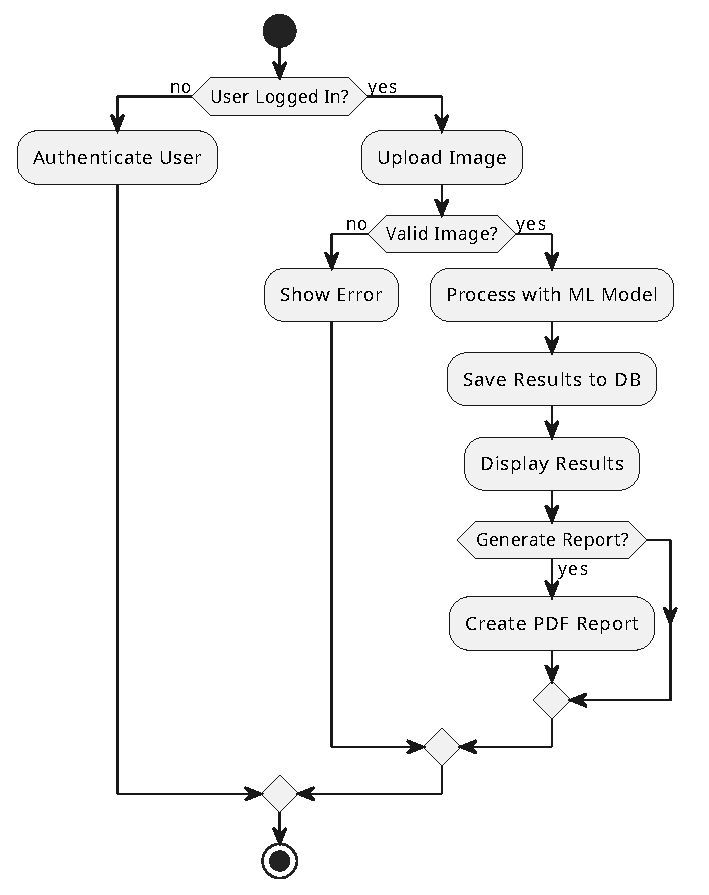
\includegraphics[width=0.70\linewidth]{Images/Highlevel/activity.pdf}
                  \caption{Activity Diagram}
                  \label{fig:ActivityDiagram}
              \end{figure}
          \end{center}
          The activity diagram outlines the decision-based workflow of the application. The process starts with authentication verification, directing unauthenticated users through the login process before proceeding. Once authenticated, users can upload images, which undergo validation to ensure they meet the system requirements for format and size. Valid images proceed to ML model processing, where the deep learning algorithm analyzes the brain scan for tumor detection. Successful analysis results are saved to the database and displayed to users. The workflow includes an optional branch for PDF report generation, allowing users to create downloadable documentation of their analysis results. Error handling is integrated throughout, redirecting users to appropriate error states when validation or processing fails.
\end{enumerate}
